% unofficial poster template for Trinity College Dublin
% which is a fork of the unofficial University of Texas at Arlington Math Poster template:
% which is a fork of the unofficial University of Lethbridge Poster template: https://www.overleaf.com/latex/templates/university-of-lethbridge-unofficial-poster-template/nddfzgvqvfwf
% which is a fork of unofficial University of Alberta Poster template: 
% which is a fork of Yale template: https://www.overleaf.com/latex/templates/yale-poster-template/rjpgqfgvsjcv
% which is a fork of the UMich template https://www.overleaf.com/latex/templates/university-of-michigan-umich-poster-template/xpnqzzxwbjzc
% which is fork of the MSU template https://www.overleaf.com/latex/templates/an-unofficial-poster-template-for-michigan-state-university/wnymbgpxnnwd
% which is a fork of https://www.overleaf.com/latex/templates/an-unofficial-poster-template-for-new-york-university/krgqtqmzdqhg
% which is a fork of https://github.com/anishathalye/gemini
% also refer to https://github.com/k4rtik/uchicago-poster
% and https://www.overleaf.com/latex/templates/tcd-poster-template/gtnrnpdmqxgk

\documentclass[final]{beamer} %FIXME SELF-REFERENCE IS SO IMPORTANT. ADDRESS IT DIRECTLY, MAYBE BRING A CARD THAT SAYS "(THIS) STATEMENT IS NOT (TRUE)" AND THIS STATEMENT IS CANNOT BE PROVED

% ====================
% Packages
% ====================

\usepackage[T1]{fontenc}
\usepackage[utf8]{luainputenc}
\usepackage{lmodern}
\usepackage[size=custom, width=122,height= 91, scale=1.2]{beamerposter} %OG size=custom, width=122,height=91, scale=1.2
\usetheme{gemini}
\usecolortheme{msu}
\usepackage{graphicx}
\usepackage{booktabs}
\usepackage{tikz}
\usepackage{pgfplots}
\pgfplotsset{compat=1.14}
\usepackage{anyfontsize}

% ====================
% Lengths
% ====================

% If you have N columns, choose \sepwidth and \colwidth such that
% (N+1)*\sepwidth + N*\colwidth = \paperwidth
\newlength{\sepwidth}
\newlength{\colwidth}
\setlength{\sepwidth}{0.025\paperwidth}
\setlength{\colwidth}{0.3\paperwidth}

\newcommand{\separatorcolumn}{\begin{column}{\sepwidth}\end{column}}

% ====================
% Title
% ====================

\title{Gödel's First Incompleteness Theorem}

\author{Bruno Cassani}
% add following line if you have co-author(s)
% Coauthor One$^{2}$, Coauthor Two$^{3}$

\institute[shortinst]{\textbf{Morrissey College of Arts and Sciences}, Boston College}

% ====================
% Footer (optional)
% ====================

\footercontent{  \hfill
  \href{mailto:cassanib@bc.edu}{cassanib@bc.edu}}
% (can be left out to remove footer)

% ====================
% Logo
% ====================

% use this to include logos on the left and/or right side of the header:
% Left: institution
 \logoright{
\includegraphics[height=8cm]{logos/bclogo.png}}
% Right: funding agencies and other affilations 
%\logoright{\includegraphics[height=7cm]{logos/NSF.eps}}

% ====================
% Body. Real Poster starts here
% ====================

\begin{document}



\begin{frame}[t]
\begin{columns}[t]
\separatorcolumn

\begin{column}{\colwidth}



  \begin{alertblock}{Theorem}

    In every reasonable axiomatic proposition of number theory, there will always be propositions that cannot be proven nor disproven.

    \begin{figure}
      \centering
            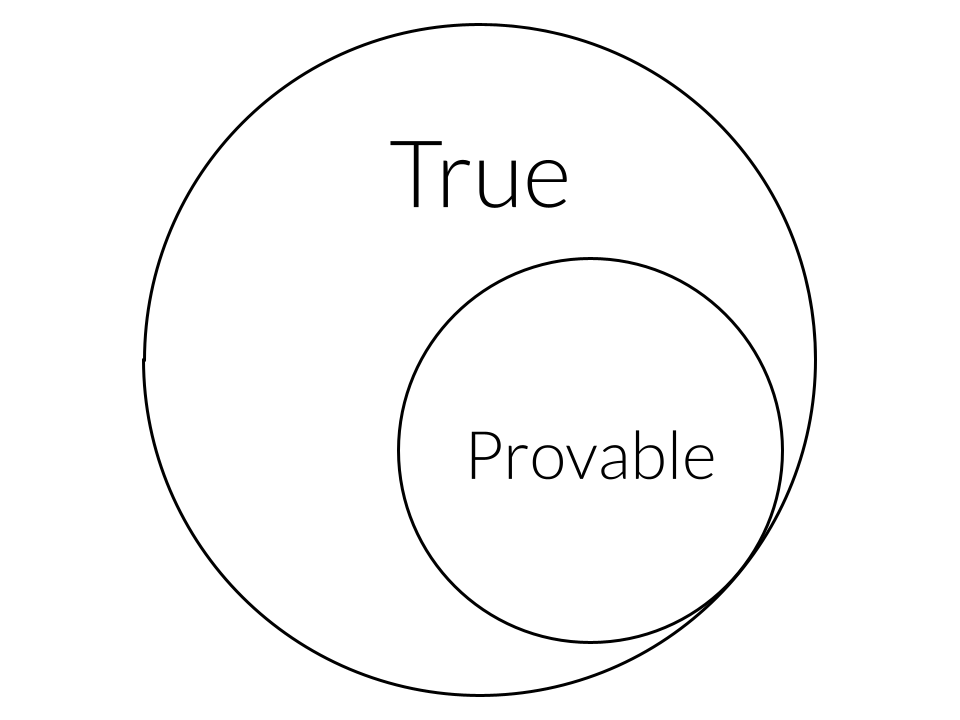
\includegraphics[width=0.5\textwidth]{figures/Draw_1.png}
    \end{figure}

  \end{alertblock}
  
\begin{block}{Background}

    \begin{itemize}
      \item Before Gödel, metamathematicians expected math to eventually be \textbf{complete}, i.e., to be able to prove everything given the right amount of axioms.
      \item In the early 20th century, set theory paradoxes like those proposed by Bertrand Russell raised questions about the \textbf{consistency} of math.
        
    \end{itemize}

\end{block}

\begin{exampleblock}{Proposition}

      Statements \textit{of} number theory could also be \textit{about} number theory.

\end{exampleblock}

\begin{block}{Gödel Numbering}

      Gödel needed math to be self-referential. First, he created his own $Encode(G)$ function to turn mathematical statements into unique natural numbers. To do so, he would first need to convert each mathematical symbol into a number.

    \begin{table}[h]
    \centering
    \begin{tabular}{c|c}
    \textbf{Constant Sign} & \textbf{Gödel Number} \\ \hline
    $\neg$ & 1 \\ 
    $\lor$ & 2 \\ 
    $\supset$ & 3 \\ 
    $\exists$ & 4 \\ 
    $=$ & 5 \\ 
    $\vdots$ & $\vdots$ \\ 
    \end{tabular}
    \end{table}

    %FIXME: LEAVE A LINE HERE?
    Through this numbering system, each symbol has its own unique natural number to be used for encoding.
    
  \end{block}

\end{column}

\separatorcolumn %NEW COLUMN%

\begin{column}{\colwidth}

  \begin{block}{Encoding}

    Given a sequence of Gödel numbers $(x_1, x_2, \dots, x_n)$, the encoding is the product of the first $n$ prime numbers raised to the values in the sequence.

    $$Encode(x_1, x_2, \dots, x_n) = 2^{x_1} \times 3^{x_2} \times \ldots \times p_n^{x_n}$$

    This way, any given mathematical expression can be encoded algebraically. Besides, the statements can be decoded through prime factorization.

    Note: $Encode(A)$ is sometimes written as $\ulcorner A \urcorner$.

  \end{block}

 \begin{block}{Provability}

Since statement A can be proved through axiom B, and $Encode(A)$ and $Encode(B)$ are unique numbers, there must be a mathematical relation between the two.

 \begin{itemize}
    
    \item We can express this relation as a function $Provability(A)$ that determines whether a statement $A$ is provable within the formal system.
    
    \item This function is essentially a binary predicate that determines if $A$ can be proved with the current axioms.
    
    \end{itemize}

 \end{block}


 \begin{block}{Self-reference by diagonalization}

    Enumerate all formulas in the formal system $F$ with exactly one free variable:
    
    \[
    \begin{array}{c|c|c|c|c}
    & n=1 & n=2 & \cdots & n = j \\
    \hline
    F_1(n) & F_1(1) & F_1(2) & \cdots & F_1(j) \\
    F_2(n) & F_2(1) & F_2(2) & \cdots & F_2(j) \\
    \vdots & \vdots & \vdots & \ddots & \vdots \\
    F_j(n) & F_j(1) & F_j(2) & \cdots & F_j(j) \\
    \end{array}
    \]


Each entry represents a formula \( F_i(n) \), where \( i \) represents the formula number and \( n \) represents the parameter.
\end{block}

\begin{block}{Gödel Statement}

Construct a new formula $G$, asserting the negation of provability for each formula $F_j(j)$ in the table:
$$G \equiv \neg Provability(F_j(j))$$

Consider the truth value of $G$. If $G$ were false, then by its own definition, each $F_j(j)$ would be provable and thus true. But the definition of $G$ implies the opposite; since math is consistent, $G$ must be true. Since $G$ cannot be consistently proven or disproven within the system, it follows that $G$ is true but unprovable within $F$.
 
 \end{block}

\end{column}


%%THIRD COLUMN
\separatorcolumn

\begin{column}{\colwidth}


  \begin{block}{References}

    \nocite{*}
    \footnotesize{\bibliographystyle{plain}\bibliography{poster}}

  \end{block}

\end{column}

\separatorcolumn
\end{columns}
\end{frame}

\end{document} 
